% Created 2022-06-08 Wed 08:44
% Intended LaTeX compiler: pdflatex
\documentclass[letter]{article}
\usepackage[utf8]{inputenc}
\usepackage[T1]{fontenc}
\usepackage{graphicx}
\usepackage{grffile}
\usepackage{longtable}
\usepackage{wrapfig}
\usepackage{rotating}
\usepackage[normalem]{ulem}
\usepackage{amsmath}
\usepackage{textcomp}
\usepackage{amssymb}
\usepackage{capt-of}
\usepackage{hyperref}
\usepackage{multicol}
\usepackage[margin=1.3in]{geometry}
\setlength{\columnsep}{1cm}
\usepackage{mathptmx}
\fontfamily{ppl}\selectfont
\usepackage[spanish, noindentfirst]{babel}
\usepackage{setspace}
\setstretch{1.5}
\usepackage{fancyhdr}
\fancyhf{}
\pagestyle{fancy}
\lhead{\hleft}
\rhead{\hright}
\cfoot{\thepage}
\renewcommand{\headrulewidth}{1pt}
\renewcommand{\footrulewidth}{0pt}
\newcommand{\hleft}{Segundo Parcial INF 354}
\newcommand{\hright}{Jesus Rodolfo Izurieta Veliz}
\setlength{\parindent}{0em}
\author{Jesus Rodolfo Izurieta Veliz}
\date{\today}
\title{Segundo Parcial INF 354}
\hypersetup{
 pdfauthor={Jesus Rodolfo Izurieta Veliz},
 pdftitle={Segundo Parcial INF 354},
 pdfkeywords={},
 pdfsubject={},
 pdfcreator={Emacs 28.1 (Org mode 9.5)}, 
 pdflang={Spanish}}
\begin{document}

\maketitle


\section{Segundo examen parcial INF 354}
\label{sec:org39f43a8}

Jesus Rodolfo Izurieta Veliz

\textbf{Repositorio:} \url{https://github.com/izurietajr/segundo-parcial/tree/master}

\begin{enumerate}
\item Generar una red neuronal (sin librerias) que utilice el daatset iris con
producto punto, errores, y de dos capas.

\item Dado la función f(x) en excel realice al menos tres generaciones del
funcionamiento del algoritmo genético.

\item Dado el siguiente grafo, Generar el archivo CSV, obtener el mejor recorrido
usando algoritmos genéticos sin el uso de DEAP.

\begin{center}
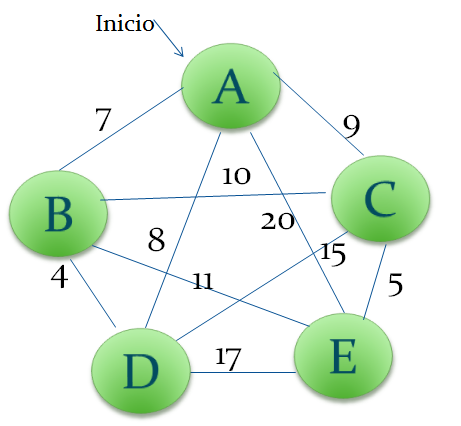
\includegraphics[width=.9\linewidth]{./graph.png}
\end{center}

\item Con el uso de DEAP, resolver el anterior ejercicio.

\item Generar un agente inteligente que diferencia dos cadenas de caracteres.
\end{enumerate}

Cada pregunta debe ser almacenada en Github o Colab o Kaagle, la misma permitir
su acceso minimamente a msilva@fcpn.edu.bo. Adjuntar el link por pregunta en un
PDF o Word y enviarlo para su revisión.
\end{document}
